\section{Auswertung}
\label{sec:Auswertung}

\subsection{Bestimmung der freien Weglänge}
Zunächst werden sowohl die Sättigungsdampfdrücke $p_{\text{sätt}}$ aus \autoref{eqn:p1}, als auch die mittleren Weglängen der Elektronen aus \autoref{eqn:w1} für die verschiedenen Temperaturen,
bei denen die Versuche durchgeführt werden, bestimmt.
Die Ergebnisse sind in \autoref{tab:f0} angegeben.

\begin{table}
  \centering
  \caption{Bestimmung der Sättigungsdampfdrücke sowie der mittleren Weglängen.}
  \label{tab:f0}
  \sisetup{parse-numbers=false}
  \begin{tabular}{
  S[table-format=3.2]
  S[table-format=2.3]
  S[table-format=1.3]
  }
\toprule
{T  /  \si{\kelvin}}		& {$p_{\text{sätt}} \:/\: \si{\bar}$}		& 
{$\bar{w} \:/\: 10^{-3} \si{\metre} $}		\\ 
\midrule
  300 & 0,0061  & 474 \\
  415 & 3,505  & 0,8274 \\
  430 & 6,247  & 0,4642 \\
  445 & 10,710 & 0,2708 \\
  460 & 17,726  & 0,1636 \\
  \bottomrule
  \end{tabular}
  \end{table}
\noindent
Der Abstand zwischen Kathode und Beschleunigungselektrode beträgt bei der verwendeten Apparatur etwa $\SI{1}{\centi\metre}$.
Daraus folgt, dass die mittlere Weglänge im Mikrometerbereich liegen sollte.
Es können demnach gute Franck-Hertz-Kurven bei Temperaturen von $\SI{400}{\kelvin}$ bis $\SI{450}{\kelvin}$ aufgezeichnet werden.

%%%%%

\subsection{Integrale Energieverteilung}
\label{sec:ie}
Wie bereits in der Durchführung erläutert wird eine feste Beschleunigungsspannung von $U_b = \SI{11}{\volt}$ eingestellt und der Auffängerstrom gemessen.
Um nun die integrale Energieverteilung bestimmen zu können, müssen mehrere Spannungswerte $U_a$ gegen den dazugehörigen Wert
\begin{equation}
  \increment I_a \coloneq I_a(U_a) - I_a(U_a + \increment U_a)
\end{equation}
aufgetragen werden.
Dieser Zusammenhang beschriebt nach \autoref{eqn:beschlGl} die Energieverteilung. Eine hohe Änderung von $I_a$ entspricht einer hohen Anzahl von Elektronen,
die ebendiese kinetische Energie besitzen und nun durch die Bremsspannung aufgehalten werden.
\newline
Die Messungen wurden einmal bei Raumtemperatur und einmal bei $T = \SI{423,16}{\kelvin}$ durchgeführt. Die Ergebnisse sind für Raumtemperatur in \autoref{fig:ev1} und für
$T = \SI{423,16}{\kelvin}$ in \autoref{fig:ev2} dargestellt.

\begin{figure}[H]
	\centering
	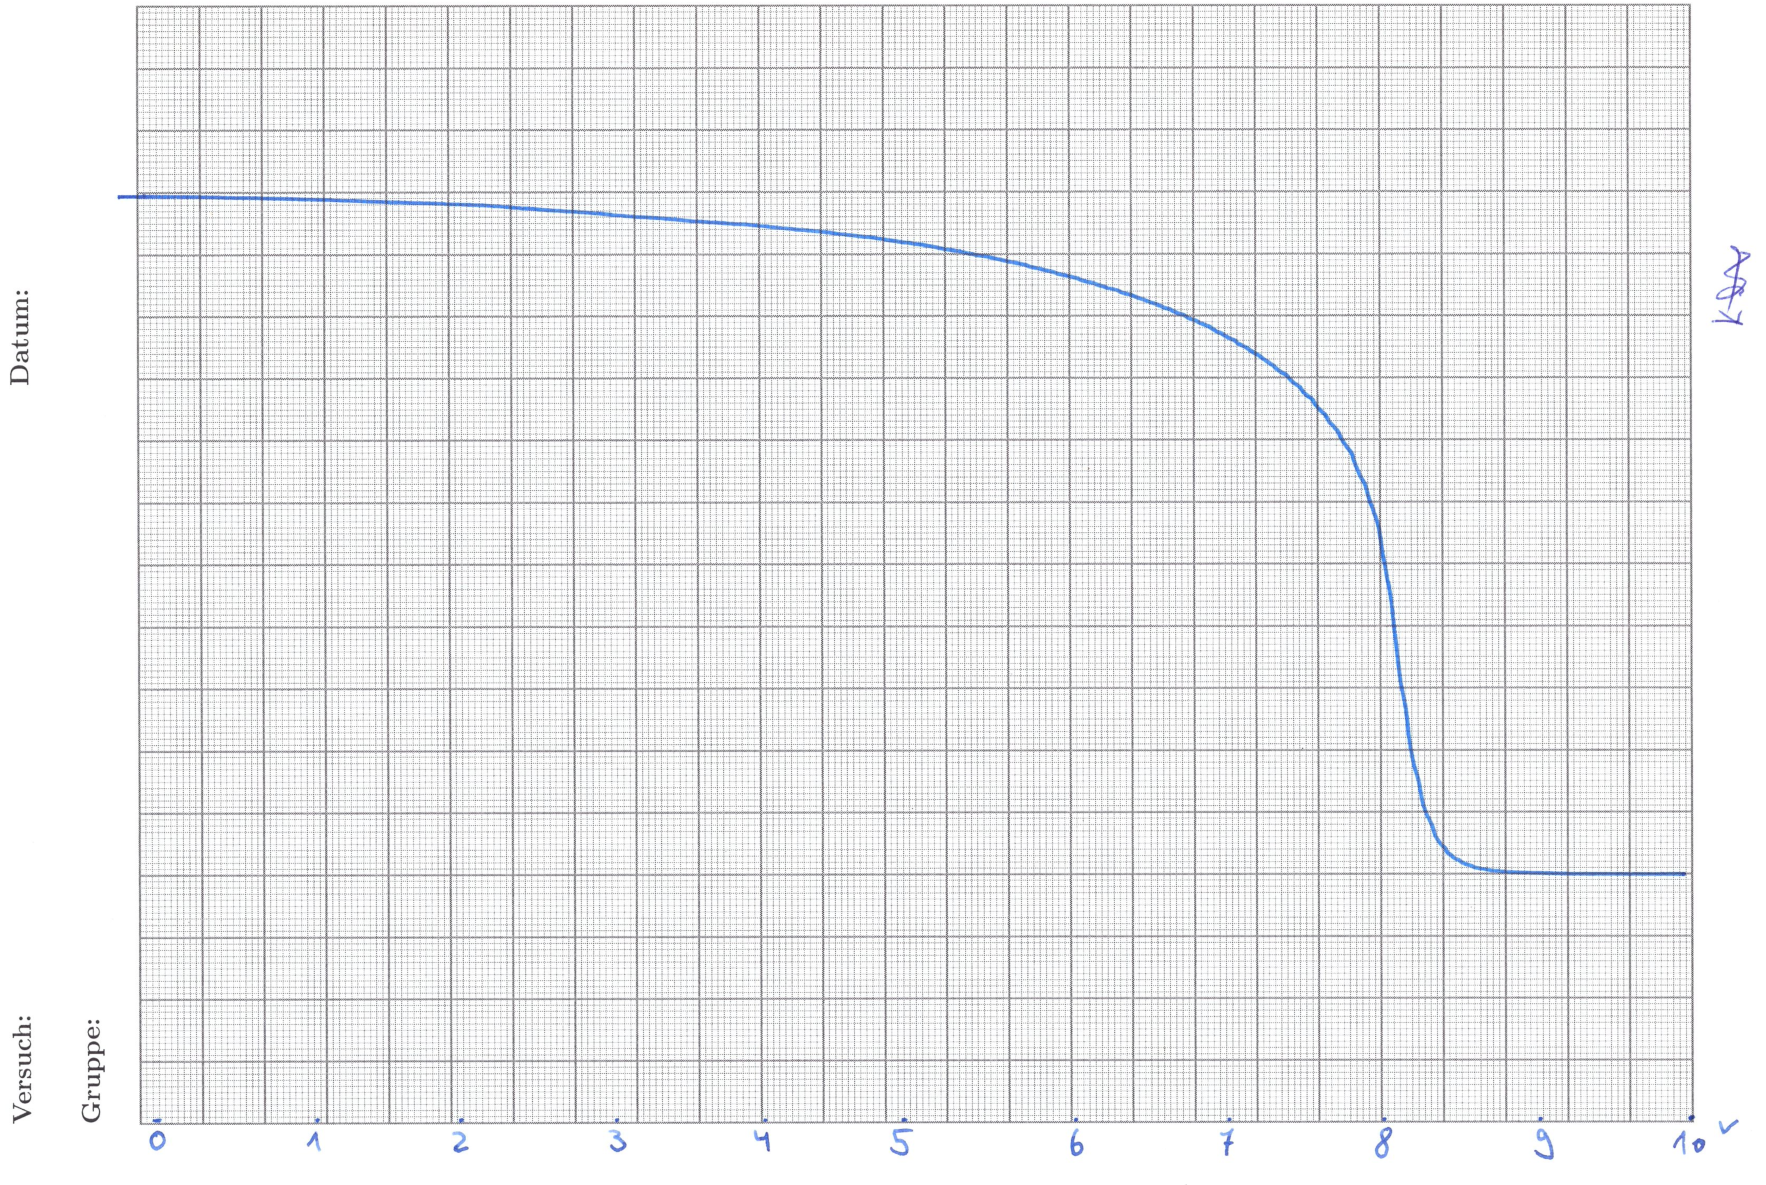
\includegraphics[width=0.7\linewidth]{data/EnergieverteilungRT.png}
	\caption{Energieverteilungsmessung bei Raumtemperatur.}
	\label{fig:ev1}
\end{figure}

\begin{figure}[H]
	\centering
	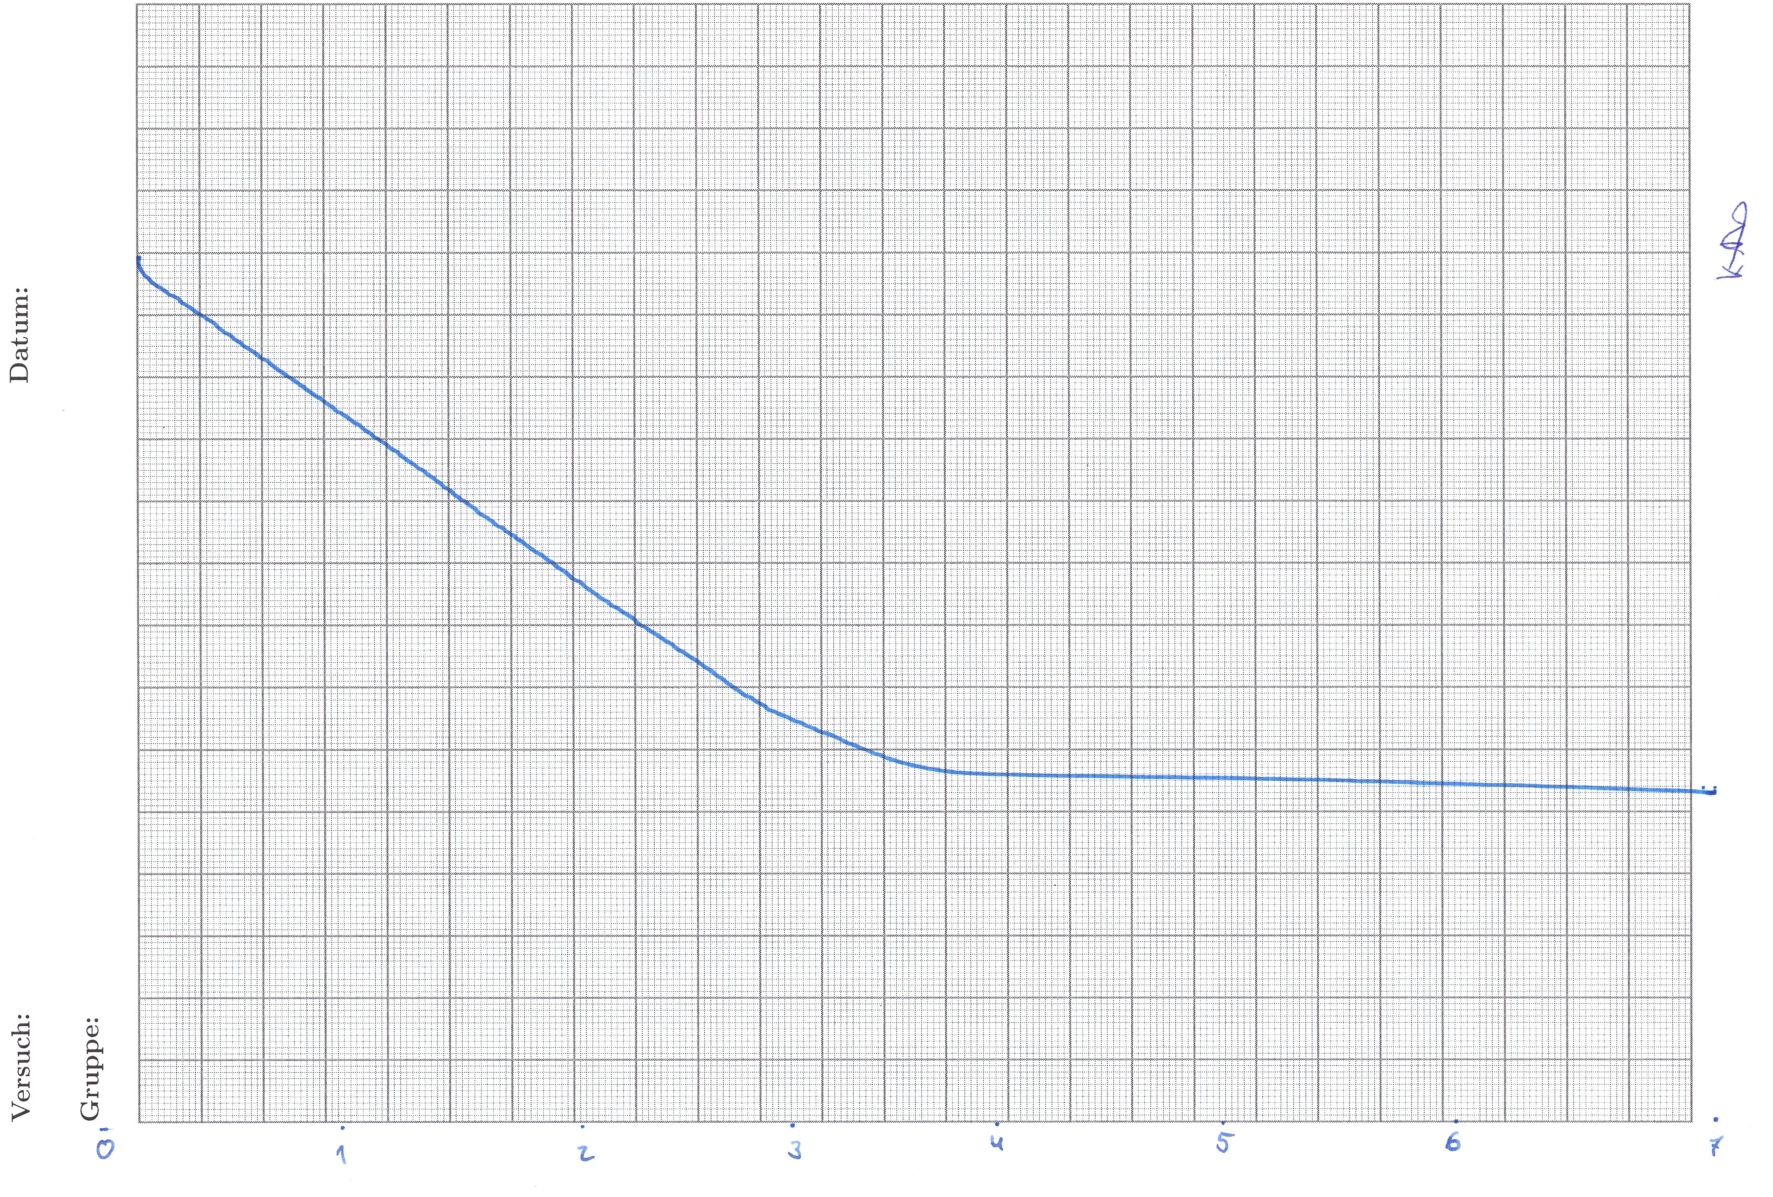
\includegraphics[width=0.7\linewidth]{data/Energieverteilung150C.png}
	\caption{Energieverteilungsmessung bei $T = \SI{423,16}{\kelvin}$.}
	\label{fig:ev2}
\end{figure}
\noindent
Beide Kurven fallen kontinuierlich, jedoch unterschiedlich stark und weisen keine Peaks auf.

\subsection{Interpretation der Franck-Hertz Kurven}
Die Franck-Hertz-Kurve bei $T = \SI{443,16}{\kelvin}$ ist in \autoref{fig:fh170} und die bei $T = \SI{463,16}{\kelvin}$ in \autoref{fig:fh190} aufgezeichnet.
\begin{figure}[H]
	\centering
	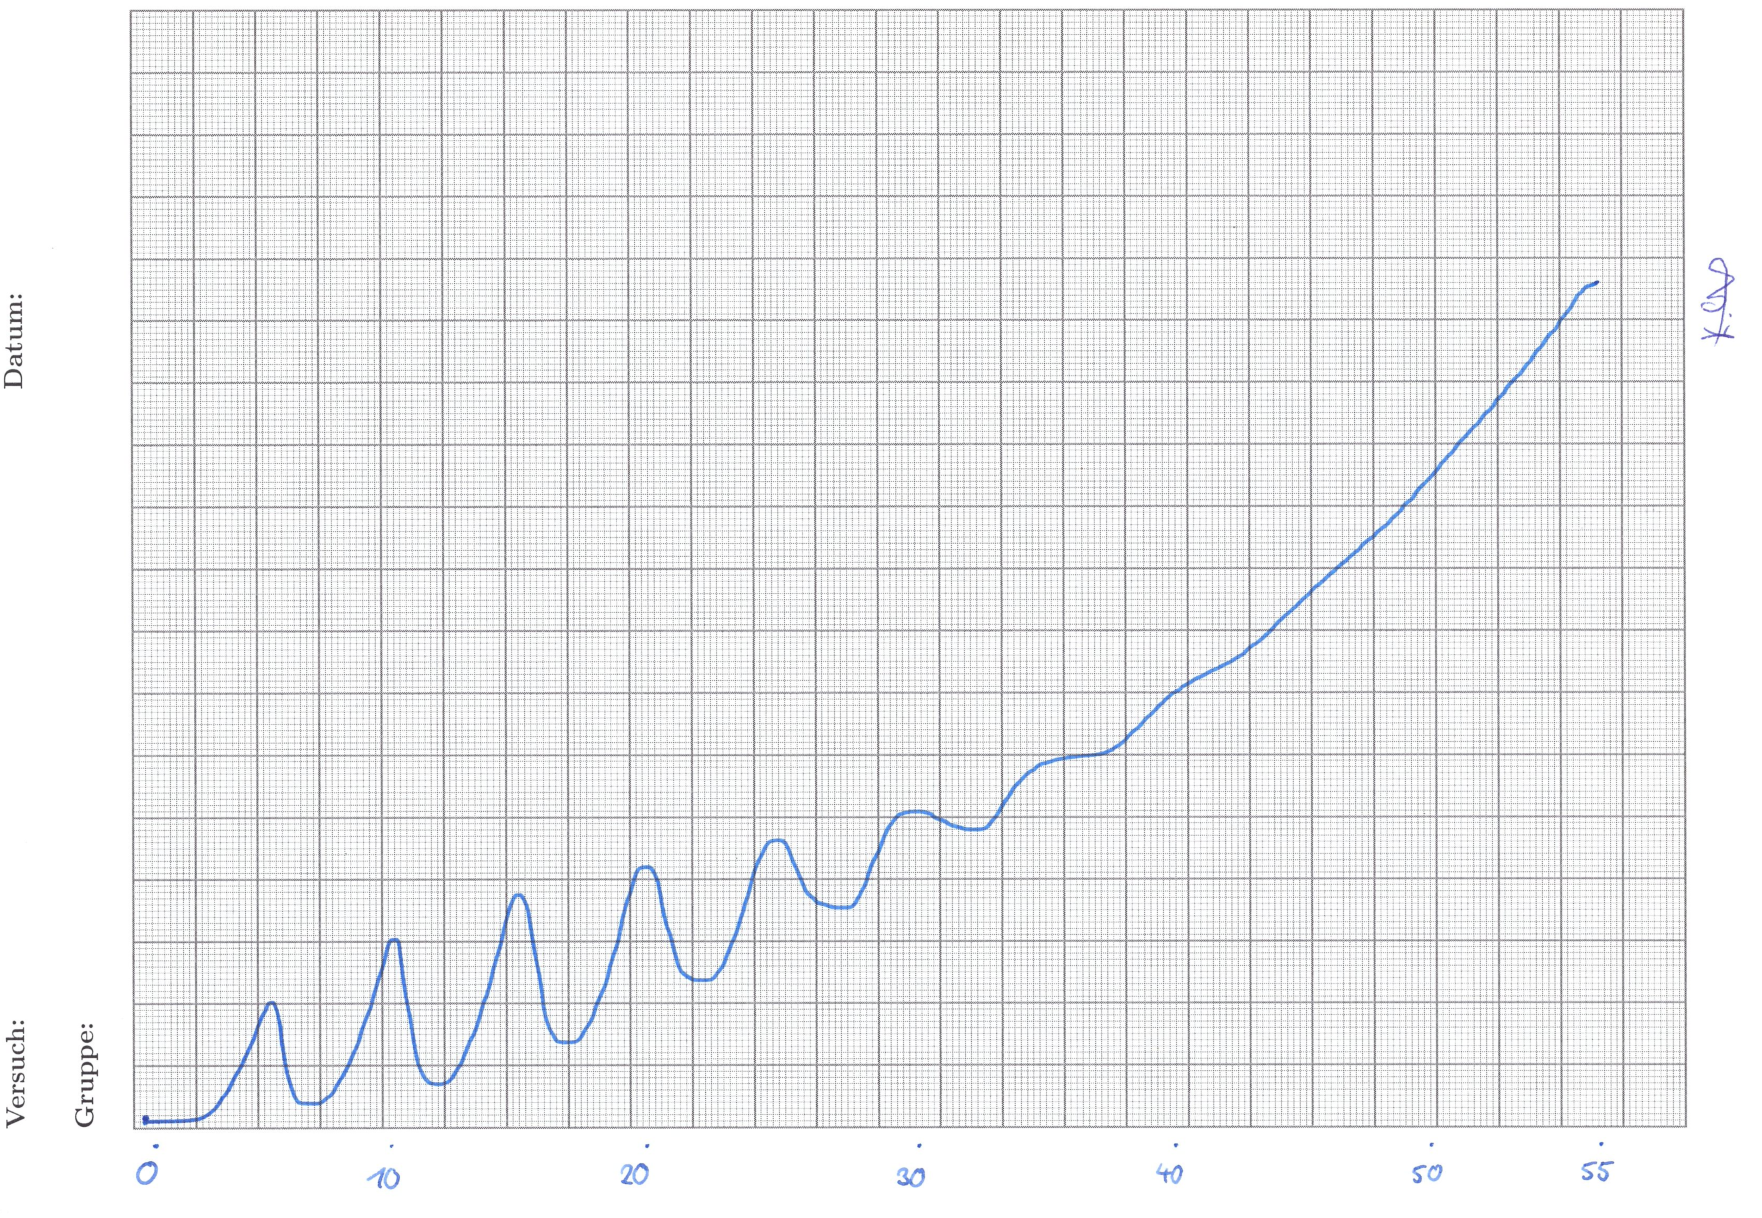
\includegraphics[width=0.7\linewidth]{data/Franck-Hertz170C.png}
	\caption{Franck-Hertz-Kurve bei $\SI{443,16}{\kelvin}$.}
	\label{fig:fh170}
\end{figure}

\begin{figure}[H]
	\centering
	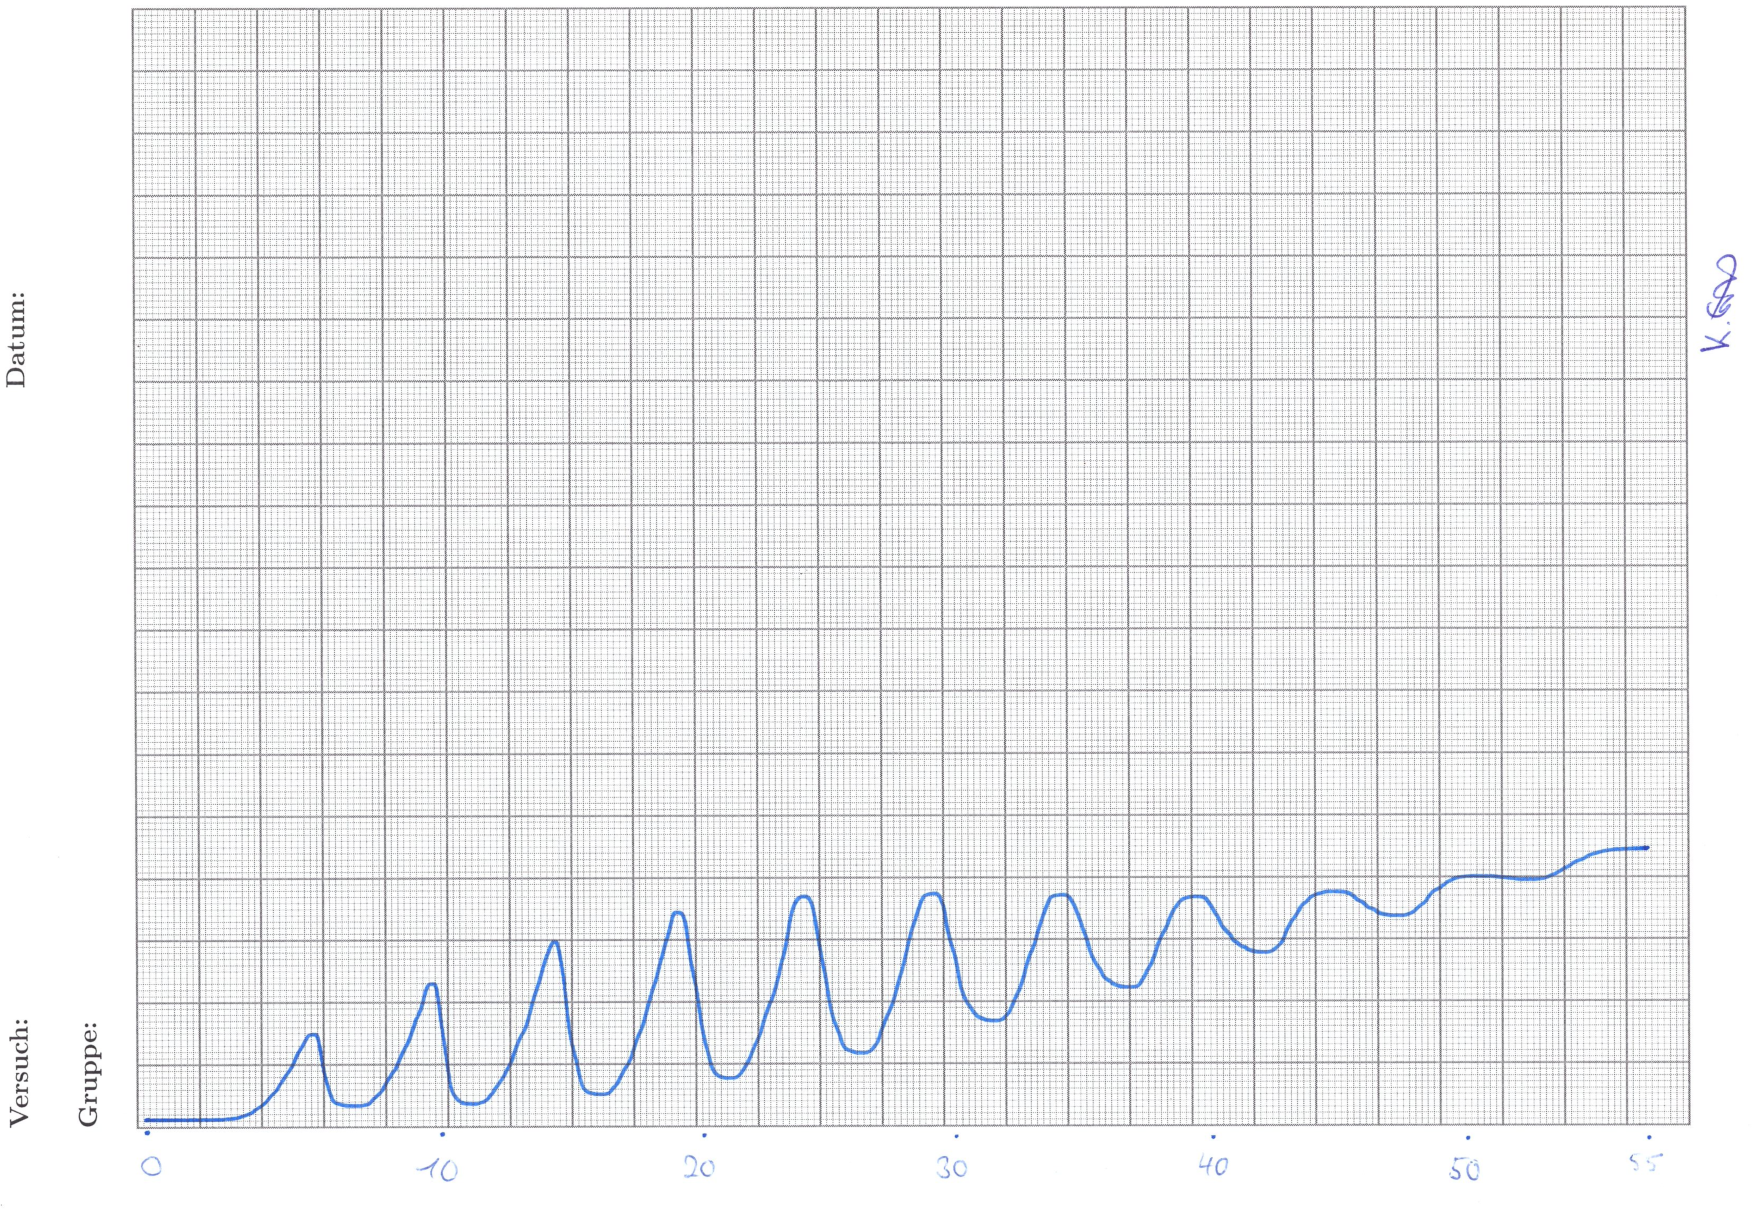
\includegraphics[width=0.7\linewidth]{data/Franck-Hertz190C.png}
	\caption{Franck-Hertz-Kurve bei $\SI{463,16}{\kelvin}$.}
	\label{fig:fh190}
\end{figure}
Es wird zur Auswertung die Franck-Hertz-Kurve bei $T = \SI{463,16}{\kelvin}$ verwendet.
Die ablesbaren Maxima befinden sich bei
\begin{align*}
  U_1 &= \SI{6,34}{\volt}, \\
  U_2 &= \SI{10,98}{\volt}, \\
  U_3 &= \SI{15,85}{\volt},\\
  U_4 &= \SI{20,73}{\volt},\\
  U_5 &= \SI{25,61}{\volt},\\
  U_6 &= \SI{30,73}{\volt}.
\end{align*}
Daraus folgt als gemittelte Abstand der Maxima
\begin{align*}
  \Delta U &= \SI{4,88 \pm 0,1}{\volt}.
\end{align*}
Nach \autoref{eqn:fh1} beträgt die Wellenlänge $\lambda$ der emittierten Strahlung
\begin{align*}
  \lambda &= \SI{254+-4}{\nano\metre}.
\end{align*}